\section{Использование поисковых систем для передачи информации}

Во времена, когда только начиналось развитие интернета, объём доступной информации был сравнительно мал, и пользователей сети было немного. На начальных стадиях развития сети, ее использовали сотрудники университетов и исследовательских лабораторий для обмена информацией между учреждениями.

Первым способом организации и систематизации доступа к информационным ресурсам стало создание каталогов сайтов. В них стали группировать ссылки согласно определенной тематике.

С течением времени интернет набирал популярность и количество сайтов в нем росло быстрыми темпами и каталоги разрастались с неимоверной скоростью. Кроме того данный способ структурирования интернет-ресурсов был не удобен в поиске конкретной информации, поскольку предоставлял доступ только к списку сайтов, а не их содержимого.

В 1994 году появилась первая поисковая система WebCrawler, которая позволяла искать по интернет-ресурсам требуемую информацию и выводила ее пользователям на экран.

До сих пор поисковые системы не утратили своей актуальности. С каждым днем появляются десятки новых сайтов. Для удобства управления своими ресурсами данные системы ввели средства <<Вебмастера>>, позволяющие получить информацию об индексировании сайта и поисковых запросов к нему.

Возникает предположение, что через данные легетимные поисковые системы можно организовать скрытый канал передачи информации, используя средства <<Веб-мастера>> и функцию <<Поиск для сайта>>, предоставляемую почти каждой поисковой системой.

При реализации данного канала в поисковой системе Яндекс был зарегистрирован сайт proxy.myprogram.us и была подключена к нему услуга <<Поиск для сайта>>, предоставившая уникальную ссылку на поисковую систему, из результатов поиска которой исключались все ресурсы, кроме proxy.myprogram.us. Для передачи информации разработано программное обеспечение, которое всю, передаваемую через данный канал, шифровало методом сдвига, разбивало на порции по 100 символов и полученные строки интерпретировало как поисковый запрос к поисковой системе Яндекс.

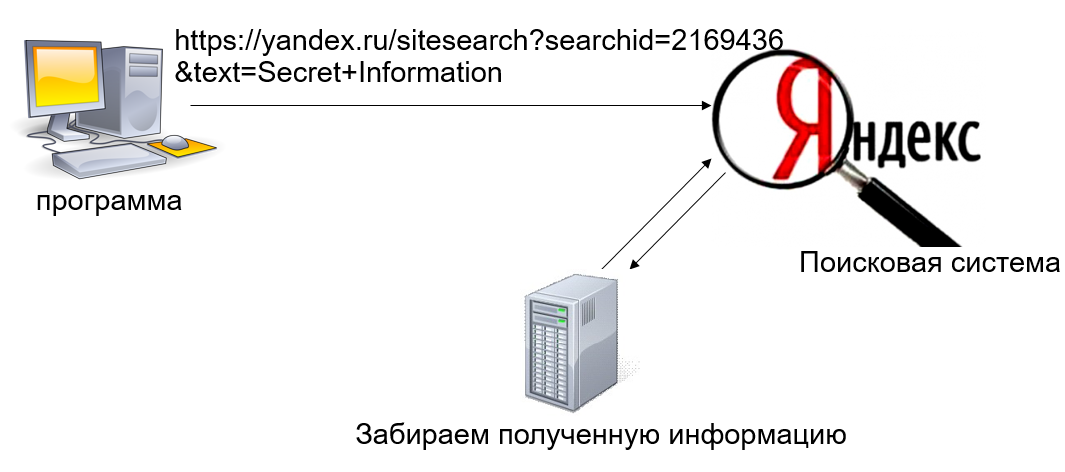
\includegraphics[width=1\linewidth]{3--yandex.png}

Тестирование данного канала имело бы успех, если бы DLP система не детектировала попытку установления защищенного соединения через SSL с поисковой системой. Firewall не блокировал соединение, но выдавал предупреждение администратору системы о том, что неизвестная программа пытается установить соединение с поисковой системой. Если не обращать на данное предупреждение внимание, то в остальном передача информации через поисковую систему Яндекс была успешной.